\documentclass[tikz,border=5pt]{standalone}
\usepackage{amsmath}
\definecolor{curveblue}{HTML}{245C86}
\begin{document}
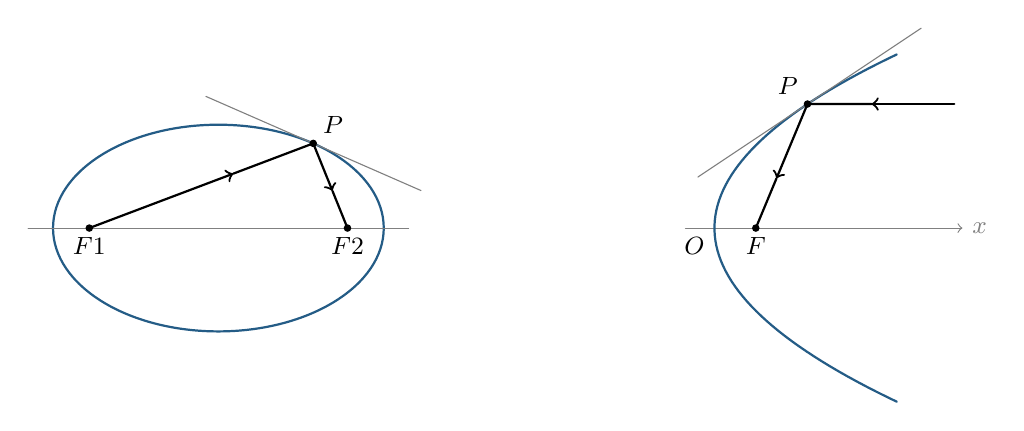
\begin{tikzpicture}[font=\small,line cap=round,scale=1.05]
\begin{scope}
\draw[curveblue,thick](0,0)ellipse[x radius=2,y radius=1.25];
\coordinate(F1)at(-1.56125,0);\coordinate(F2)at(1.56125,0);\coordinate(P)at(1.14715,1.02394);
\draw[gray](-2.3,0)--(2.3,0);
\draw[thick,->](F1)--(.18,.658);
\draw[thick](.18,.658)--(P);
\draw[thick,->](P)--(1.38,.449);
\draw[thick](1.38,.449)--(F2);
\draw[gray](-.15,1.592)--(2.45,.454);
\foreach \N/\pos in {F1/below,F2/below,P/above right}{\fill(\N)circle(1.3pt)node[\pos]{$\N$};}
\end{scope}
\begin{scope}[xshift=6cm]
\draw[gray,->](-.35,0)--(3,0)node[right]{$x$};
\draw[curveblue,thick,domain=-2.1:2.1,samples=70]plot({\x*\x/2},{\x});
\coordinate(F)at(.5,0);\coordinate(P)at(1.125,1.5);
\draw[gray](-.2,.617)--(2.5,2.417);
\draw[thick,->](2.9,1.5)--(1.9,1.5);\draw[thick](1.9,1.5)--(P);
\draw[thick,->](P)--(.75,.6);\draw[thick](.75,.6)--(F);
\fill(F)circle(1.3pt)node[below]{$F$};\fill(P)circle(1.3pt)node[above left]{$P$};
\node[below left]at(0,0){$O$};
\end{scope}
\end{tikzpicture}
\end{document}
